\documentclass[../analysisII_notes.tex]{subfiles}
\begin{document}
\section{Aula 04 - 12 de Março, 2025}
\subsection{Motivações}
\begin{itemize}
	\item Exemplos dos Conceitos Anteriores;
	\item Integrais Superior e Inferior.
\end{itemize}
\subsection{Integrais Superiores e Inferiores - Parte 2}
Na aula de hoje, observaremos exemplos e resultados a partir do desenvolvimento na aula anterior, junto à definição das integrais superior e inferior.

\hypertarget{fexample}{\begin{example}}
	Seja c uma constante real e \(f:[a, b]\rightarrow \mathbb{R}\) uma função constante e igual à c:
	\[
		f(x) = c,\quad \forall x\in [a, b].
	\]
	Forneceremos uma partição qualquer e calcularemos as somas previamente mencionadas; sendo \(\mathcal{P}\) esta partição,
	\[
		\mathcal{P}: a = t_{0} < t_1 < \dotsc < t_{n} = b,
	\]
	temos, por definição,
	\[
		M_{i}=\sup_{}\{f(x): x\in [t_{i-1}, t_{i}]\} = c,\quad \forall 0\leq i\leq n.
	\]
	Analogamente,
	\[
		m_{i} = \inf_{}{f(x):x\in [t_{i-1}, t_{i}]} = c,\quad \forall 0\leq 1\leq n.
	\]
	Assim, para todo i natural entre 1 e n, segue que \(m_{i} = M_{i} = c,\) donde temos
	\[
		U(f; \mathcal{P}) = \sum\limits_{i=1}^{n}c(t_{i}-t_{i-1}) = c \sum\limits_{i=1}^{n}(t_{i}-t_{i-1}) = c(b-a)
	\]
	e
	\[
		L(f; \mathcal{P}) =\sum\limits_{i=1}^{n}c(t_{i}-t_{i-1}) = c \sum\limits_{i=1}^{n}(t_{i}-t_{i-1}) = c(b-a).
	\]
	\begin{figure}[H]
		\begin{center}
			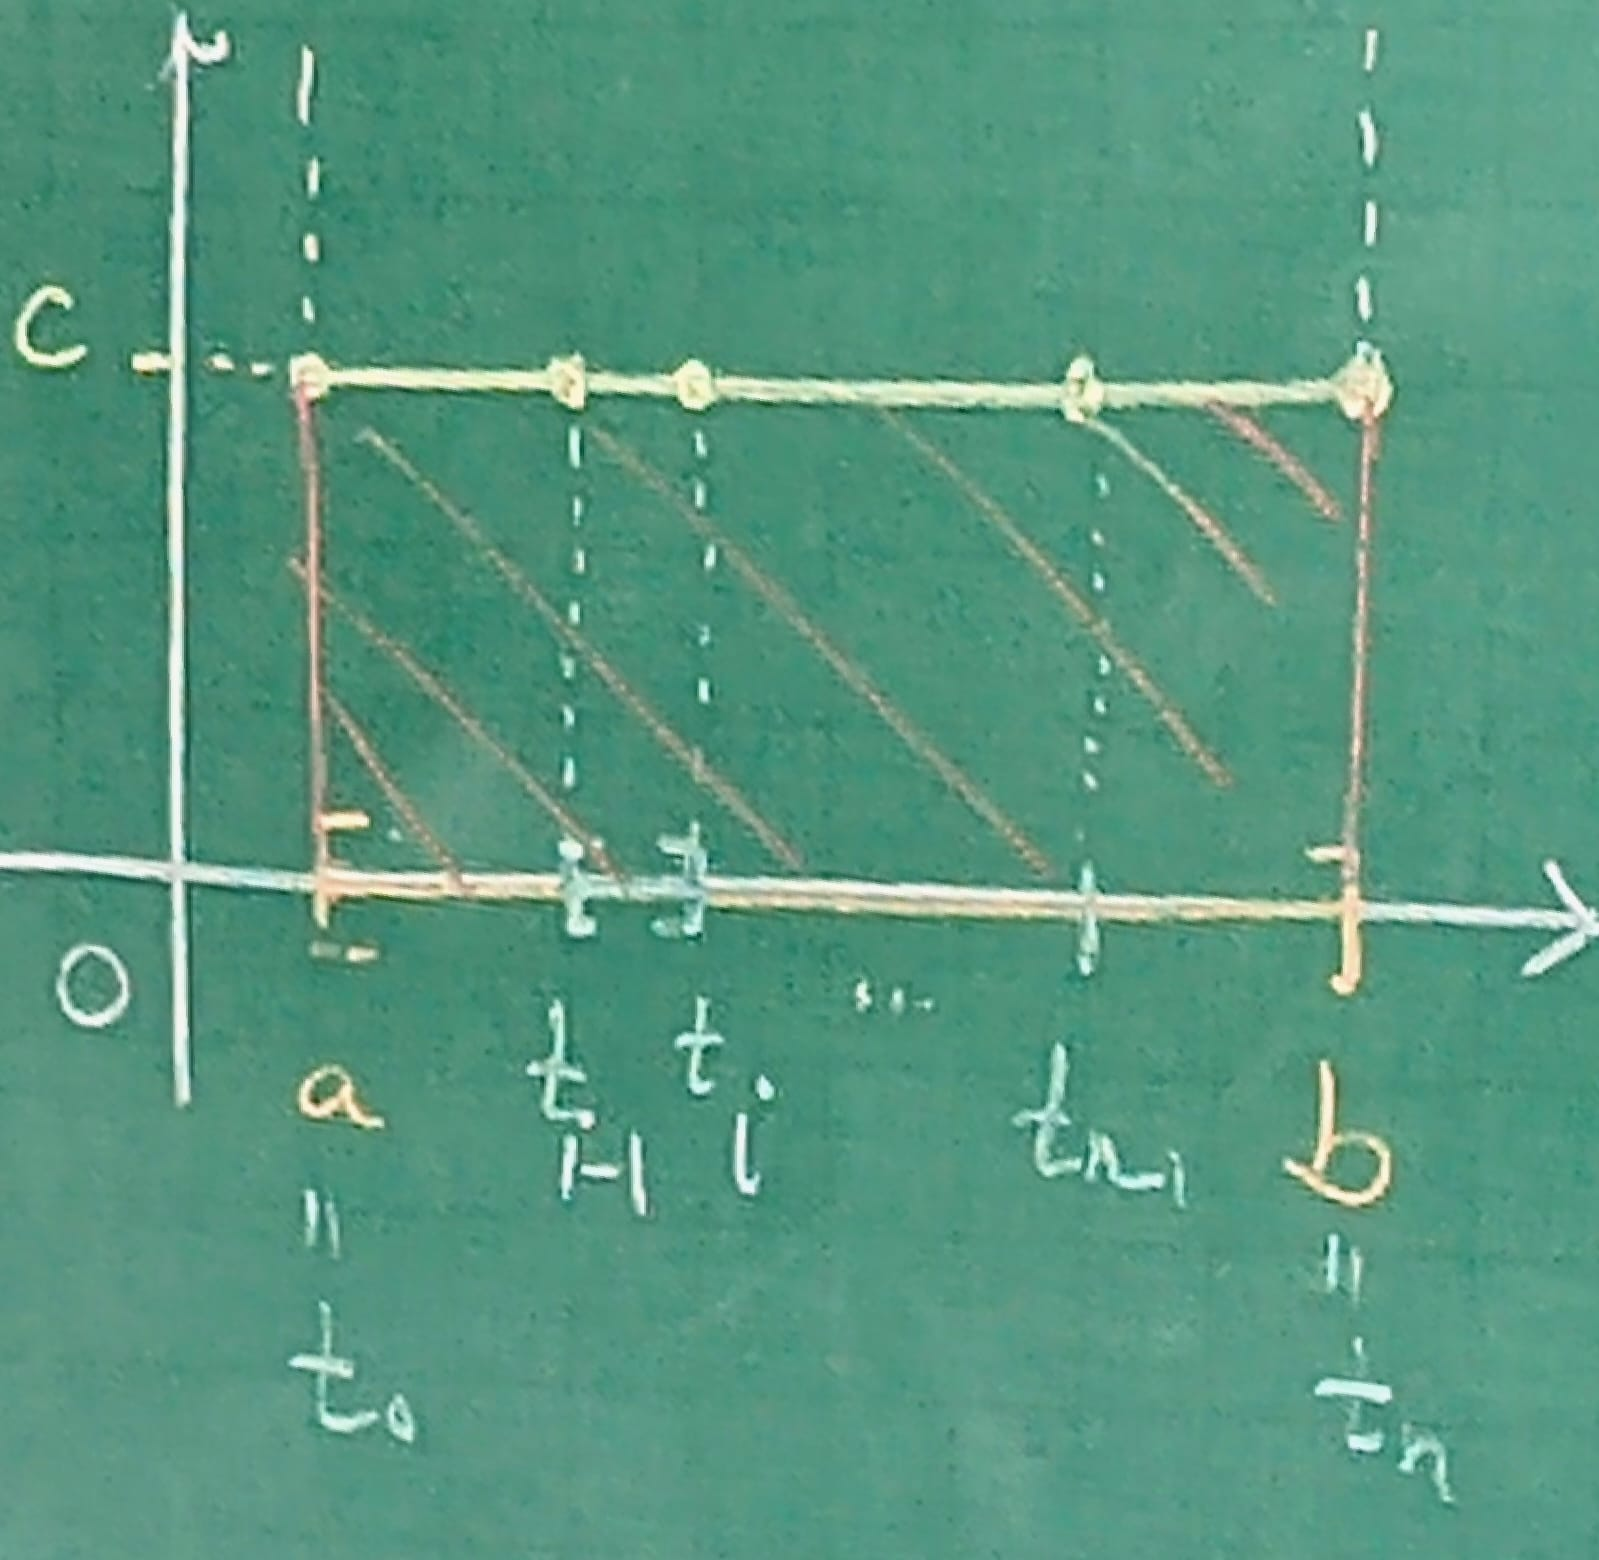
\includegraphics[height=0.5\textheight, width=0.5\textwidth, keepaspectratio]{./Images/constant_04.png}
		\end{center}
		\caption{Ilustração do intervalo \([a, b]\) particionado por \(\mathcal{P}\) e com a função constante.}
		\label{constant04}
	\end{figure}

	Em conclusão,
	\[
		\sigma (f) = \{c(b-a)\} = \Sigma (f).
	\]
\end{example}
\hypertarget{gexample}{\begin{example}}
	Agora, considere duas constantes distintas, denotadas por \(c\) e \(\alpha \), e uma função \(g:[a, b]\rightarrow \mathbb{R}\) dada por
	\[
		g(x)  = \left\{\begin{array}{ll}
			c,\quad x\in [a, b) \\
			\alpha , \quad x = b.
		\end{array}\right.
	\]
	Supondo que \(\alpha \) é maior que c e que \(\mathcal{P}\) é outra partição genérica dada por
	\[
		\mathcal{P}: a = t_{0} < t_{1} < \dotsc < t_{n} = b,
	\]
	calculamos, dado i entre 1 até o penúltimo ponto da partição (o último diferente de b, que é onde a função ``salta''), os valores
	\[
		m_{i} = \inf_{}\{g(x):x\in [t_{i-1}, t_{i}]\} = c
	\]
	e
	\[
		M_{i} = \sup_{}\{g(x):x\in [t_{i-1}, t_{i}]\} = c.
	\]
	Quando olhamos para o último ponto da partição, acontece que
	\[
		m_{n} = \inf_{}\{g(x):x\in [t_{n-1}, b]\} = \inf_{}\{c, \alpha \} = c
	\]
	e, agora sim de forma diferente,
	\[
		M_{n} = \sup_{}\{g(x):x\in [t_{n-1}, b]\} = \sup_{}\{c, \alpha \} = \alpha.
	\]

	\begin{figure}[H]
		\begin{center}
			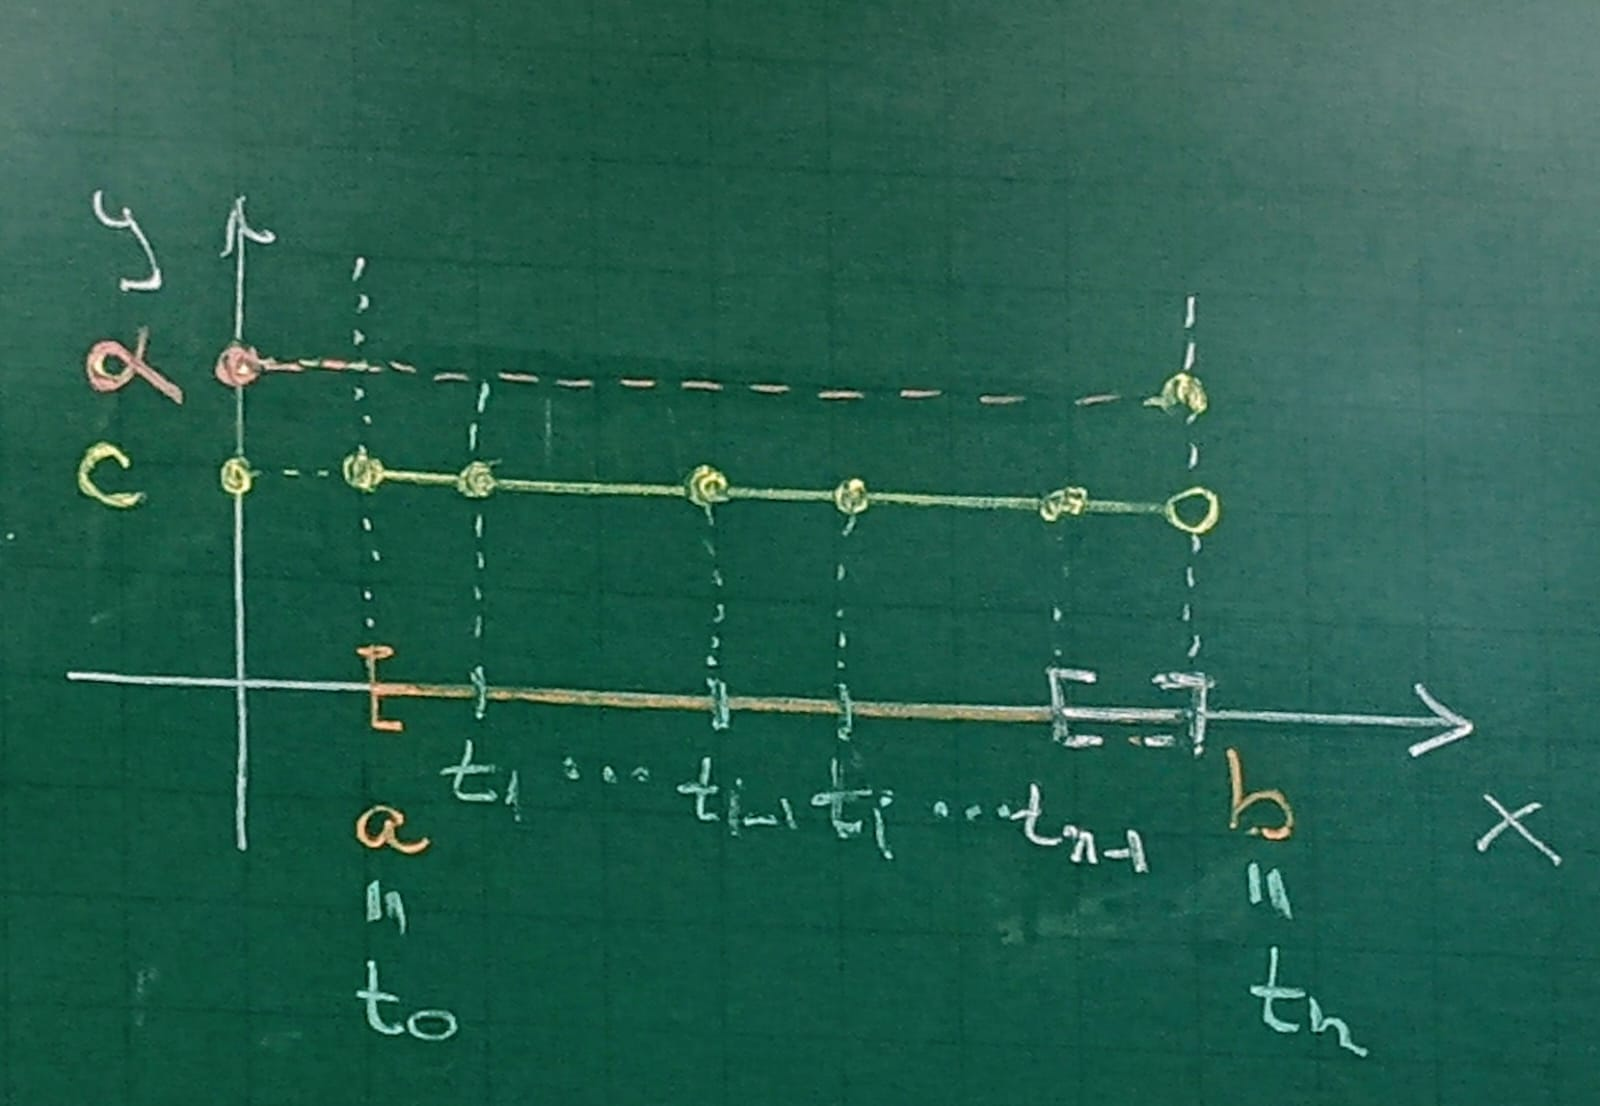
\includegraphics[height=0.6\textheight, width=0.6\textwidth, keepaspectratio]{./Images/jump_04.png}
		\end{center}
		\caption{Representação da g sobre a partição \(\mathcal{P}\) do intervalo [a, b]}
		\label{jump04}
	\end{figure}

	Logo, a soma inferior não muda
	\[
		L(g; \mathcal{P}) = \sum\limits_{i=1}^{n}m_{i}(t_{i}-t_{i-1}) = c(b-a),
	\]
	mas a superior pode mudar; vejamos se isto ocorre:
	\[
		U(g; \mathcal{P}) = \sum\limits_{i=1}^{n-1}M_{i}(t_{i}-t_{i-1}) + M_{n}(b-t_{i-1}) = c(t_{n-1} - a) + \alpha(b-t_{n-1}),
	\]
	que é uma expressão bem mais feia. O que podemos fazer é somar 0 de uma forma esperta - neste caso, somando e subtraindo b - para obter a expressão abaixo, separada em um termo dependente da partição e outro não
	\begin{align*}
		U(g; \mathcal{P}) & = c(t_{n-1} - a) + \alpha(b-t_{n-1})         \\
		                  & = c(b-a) + c(t_{n-1}-b) + \alpha (b-t_{n-1}) \\
		                  & = c(b-a) + (\alpha -c)(b-t_{n-1}).
	\end{align*}
	Curiosamente, ele depende apenas do penúltimo elemento da partição, o que permite que a partição tenha apenas três pontos!
\end{example}
\hypertarget{dirichlet}{\begin{example}[Função de Dirichlet]}
	A função de Dirichlet é \(h:[0, 1]\rightarrow \mathbb{R}\) dada por
	\[
		h(x) = \left\{\begin{array}{ll}
			1,\quad x\in \mathbb{Q}\cap [0, 1] \\
			0,\quad x\not\in \mathbb{Q}\cap [0, 1].
		\end{array}\right.
	\]
	Assim como antes, tentaremos calcular as somas inferior e superior para h; nesta linha, defina a partição
	\[
		\mathcal{P}: a = t_{0} < t_{1} < \dotsc < t_{n} = b.
	\]
	Então,
	\[
		m_{i} = \inf_{}\{h(x):x\in[t_{i-1}, t_{i}]\} = \inf_{}\{0, 1\} = 0
	\]
	e
	\[
		M_{i} = \sup_{}\{h(x):x\in[t_{i-1}, t_{i}]\} = \sup_{}\{0, 1\} = 1.
	\]
	Consequentemente,
	\begin{align*}
		 & U(h; \mathcal{P}) = \sum\limits_{i=1}^{n}(t_{i}-t_{i-1}) = 1   \\
		 & L(h; \mathcal{P}) = \sum\limits_{i=1}^{n}0(t_{i}-t_{i-1}) = 0.
	\end{align*}
	Em conclusão,
	\[
		\sigma (h) = \{0\} \quad\&\quad \Sigma (h) = \{1\}.
	\]
\end{example}
Agora, armados com estes exemplos, podemos acrescentar um corolário ao teorema da aula passada:
\begin{crl*}
	Se \(\mathcal{P}\) e \(\mathcal{Q}\) são duas partições do intervalo \([a, b]\), então
	\[
		L(f; \mathcal{P}) \leq U(f;\mathcal{Q}).
	\]
\end{crl*}
\begin{proof*}
	Com efeito, basta notar que, chamando de \(\mathcal{R}\) a partição composta da união das partições \(\mathcal{P}\) e \(\mathcal{Q}\), nota-se que ela refina tanto \(\mathcal{P}\) quanto \(\mathcal{Q}\). Logo, valem as desigualdades
	\begin{align*}
		L(f; \mathcal{P}) & \leq L(f; \mathcal{P}\cup \mathcal{Q}) \\
		                  & \leq U(f; \mathcal{P}\cup \mathcal{Q}) \\
		                  & \leq U(f; \mathcal{Q}).
	\end{align*}
	Portanto,
	\[
		L(f; \mathcal{P}) \leq U(f; \mathcal{Q}).\quad \text{\qedsymbol}
	\]
\end{proof*}

Finalmente, podemos partir para as integrais! Começamos com a definição de suas ``componentes'' - a área em excesso e a área em carecer.
\begin{def*}
	Seja \(f:[a, b]\rightarrow \mathbb{R}\) uma função limitada. Definimos:
	\begin{itemize}
		\item[a)] Sua \textbf{integral inferior} pondo:
		      \[
			      \underline{\intup_{a}^{b}}f(x) dx = \underline{\intup_{a}^{b}}f = \sup_{}\sigma (f);
		      \]
		\item[b)] Sua \textbf{integral superior} por:
		      \[
			      \overline{\intup_{a}^{b}}f(x)dx = \overline{\intup_{a}^{b}}f = \inf_{}\Sigma (f).
		      \]
	\end{itemize}
	\begin{figure}[H]
		\begin{center}
			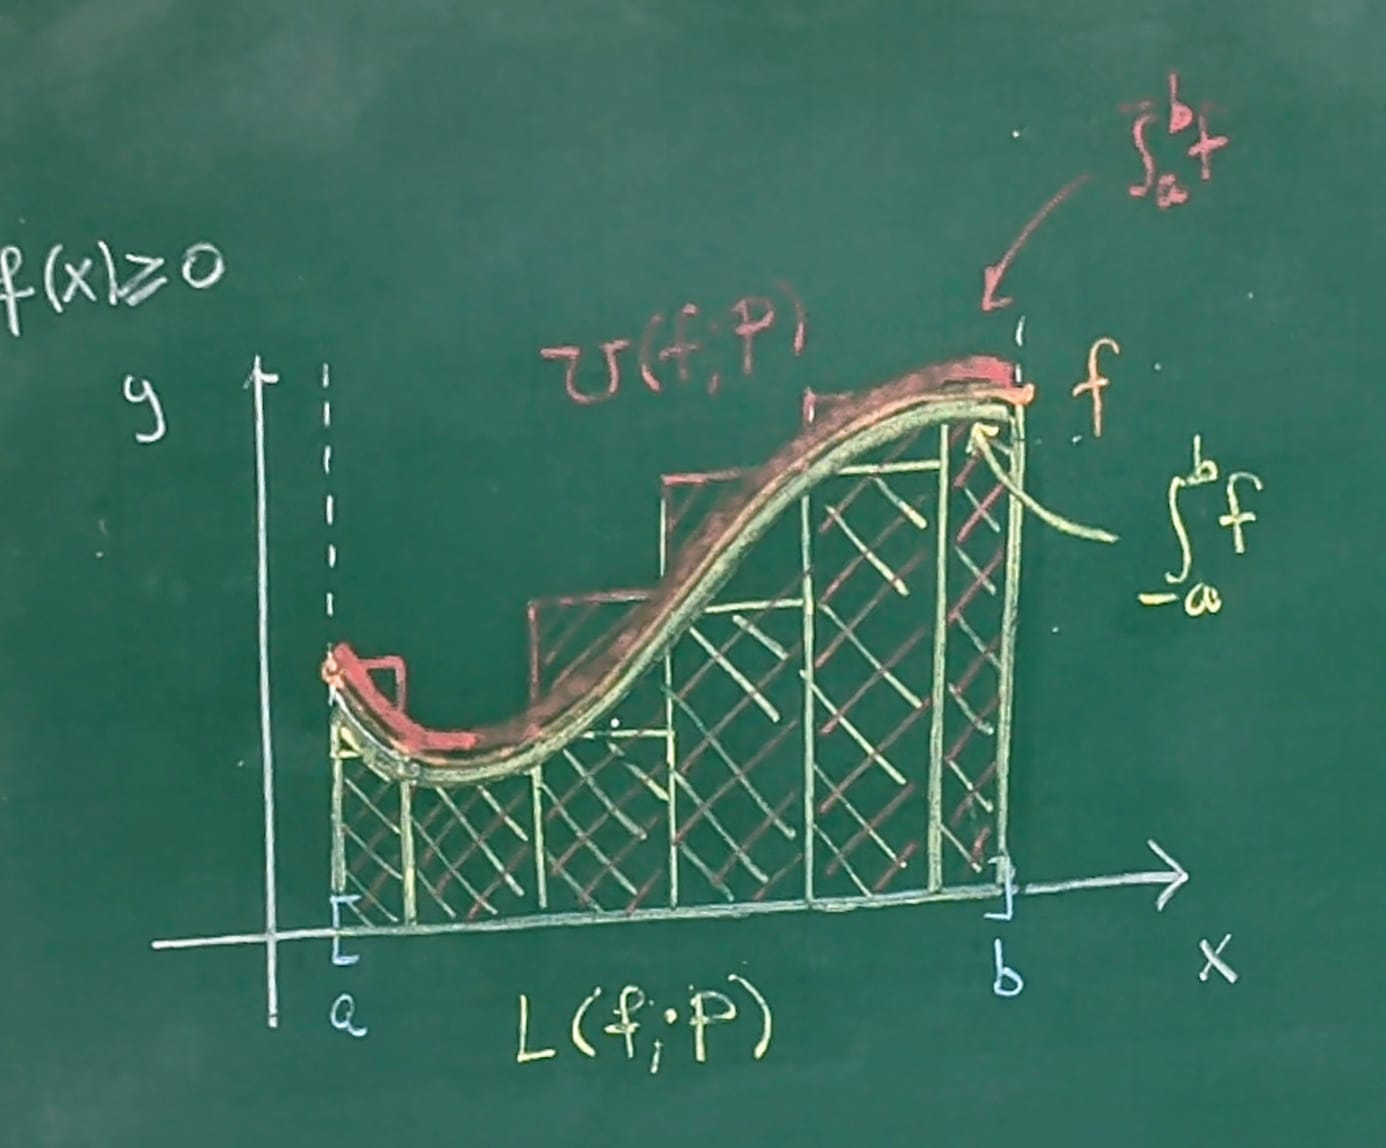
\includegraphics[height=0.6\textheight, width=0.6\textwidth, keepaspectratio]{./Images/ulint_04.png}
		\end{center}
		\caption{Integral superior (``peca pelo excesso'') e integral inferior (``peca pela falta'') da função f}
		\label{ulint04}
	\end{figure}

	Finalmente, diremos que f é \textbf{Riemann-integrável em }\([a, b]\), denotado por \(f\in \mathcal{R}([a, b])\), quando
	\[
		\underline{\intup_{a}^{b}}f = \overline{\intup_{a}^{b}}f.
	\]
	Neste caso, o valor é chamado \textbf{a integral de f em }\([a, b]\), indicado por
	\[
		\int_{a}^{b}f(x)dx = \int_{a}^{b}f = \underline{\intup_{a}^{b}}f = \overline{\intup_{a}^{b}}f.\quad \square
	\]
\end{def*}

Reaproveitando os exemplos das somas, incluindo as notações de f, g e h, veremos alguns exemplos de funções integráveis e uma que não é integrável.
\begin{example}
	\begin{itemize}
		\item[1)] \hyperlink{fexample}{\textit{Para a f}}, concluímos que
		      \[
			      \sigma (f) = \Sigma (f) = \{c(b-a)\}.
		      \]
		      Logo,
		      \[
			      \underline{\intup_{a}^{b}}f = \sup_{}\sigma (f) = \sup_{}\{c(b-a)\} = c(b-a)
		      \]
		      e
		      \[
			      \overline{\intup_{a}^{b}}f = \inf_{}\Sigma (f) = c(b-a).
		      \]
		      Portanto, f é integrável e, além disso,
		      \[
			      \int_{a}^{b}f(x)dx = c(b-a).
		      \]
		\item[2)] \hyperlink{gexample}{\textit{Para a função g}}, nota-se que
		      \[
			      \sigma (g) = \{c(b-a)\} \Rightarrow \underline{\intup_{a}^{b}}g = c(b-a).
		      \]
		      Por outro lado, se
		      \[
			      \mathcal{P}:a = t_{0} < t_{1} < \dotsc < t_{n} = b
		      \]
		      for uma partição qualquer, isto implicou em
		      \[
			      U(g; \mathcal{P}) = c(b-a) + (\alpha -c)(b-t_{n-1}),
		      \]
		      de forma tal que
		      \[
			      \Sigma (g) = \inf_{\mathcal{P}\in \mathcal{P}([a, b])}\{U(g; \mathcal{P})\}.
		      \]

		      Para calcular este ínfimo, observe que
		      \[
			      U(g; \mathcal{P}) = c(b-a) + \underbrace{(\alpha -c)(b-t_{n-1})}_{>0} > c(b-a),
		      \]
		      ou seja, c(b-a) é a cota inferior de \(\Sigma (g)\), que é a maior pois, dado \(\varepsilon > 0\), podemos escolher um ponto \(t_{1}\) entre a e b tal que
		      \[
			      b-t_{1} < \frac{\varepsilon }{\alpha - c},
		      \]
		      donde vemos que, para \(\mathcal{P}_{0} = \{a, t_{1}, b\}\) (que sabemos bastar pelo argumento dado no próprio exemplo), seguirá o seguinte:
		      \begin{align*}
			      U(g; \mathcal{P}_{0}) & = c(b-a) + (\alpha -c)(b-t_{1}) \\
			                            & < c(b-a) + \varepsilon.
		      \end{align*}
		      Como \(\varepsilon \) foi escolhido arbitrariamente, c(b-a) deve ser a maior cota inferior - qualquer folga a mais na cota inferior fica maior que \(U(g; \mathcal{P}_{0})\) - provando que
		      \[
			      c(b-a) = \inf_{}\Sigma (f) = \overline{\intup_{a}^{b}}g.
		      \]
		      Portanto, a integral existe, pois ambas a superior e a inferior coincidiram, permitindo concluirmos que
		      \[
			      \int_{a}^{b}g(x)dx = c(b-a) = \overline{\intup_{a}^{b}}g = \underline{\intup_{a}^{b}}g.
		      \]

		      Uma coisa legal deste exemplo é notar que a função não é contínua, mas mesmo assim é integrável!
		\item[3)] \hyperlink{dirichlet}{\textit{Para a h}}, vimos que
		      \[
			      \sigma (h) = \{0\} \quad\&\quad \Sigma (h) = \{1\},
		      \]
		      donde segue que
		      \[
			      \underline{\intup_{0}^{1}}h = \sup_{}\{0\} = 0
		      \]
		      e
		      \[
			      \overline{\intup_{0}^{1}}h = \inf_{}\{1\} = 1.
		      \]
		      Portanto, esta função \textbf{não} é integrável.
	\end{itemize}
\end{example}
\end{document}
